\def\nodeA{node [anchor=east] {$S_1$}}
\def\nodeB{node [anchor=west] {$S_2$}}
\def\nodeT{node [left=0.4cm] {\tiny $T_1$} node [right=0.4cm] {\tiny $T_2$}}
% Definition of circles
\def\firstcircle{(0,0) circle (1.5cm)}
\def\secondcircle{(0:2cm) circle (1.5cm)}
\def\thirdcircle{(0:1cm) circle (1.11cm)}

\colorlet{circle edge}{blue!50}
\colorlet{circle area}{blue!20}

\tikzset{filled/.style={fill=circle area, draw=circle edge, thick},
    outline/.style={draw=circle edge, thick}}





%Set A in B
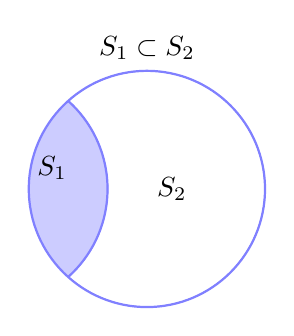
\begin{tikzpicture}
    \begin{scope}
        \clip \secondcircle;
        \draw[even odd rule,blue] \firstcircle \nodeA
                                 \secondcircle ;
                                 %\thirdcircle;
            \fill[filled] \firstcircle;
   \end{scope}
      \draw[outline] \secondcircle \nodeB;

   \node[anchor=south] at (current bounding box.north) {$S_1 \subset S_2$};
   \node[anchor=west] at (current bounding box.west) {$S_1$};
\end{tikzpicture}
%Set temporal A in B
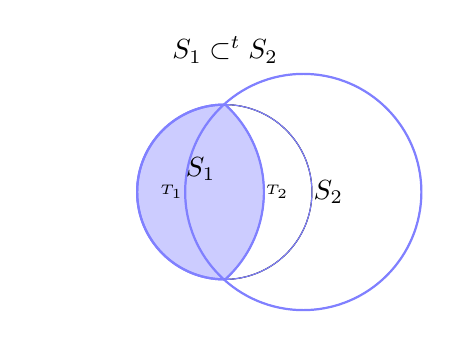
\begin{tikzpicture}
    \begin{scope}
        \clip \firstcircle;
        \fill[filled] \thirdcircle;
      \draw[outline] \thirdcircle \nodeT;
    \end{scope}
    \begin{scope}
        \clip \secondcircle;
        \draw \thirdcircle \nodeT;
    \end{scope}
      \draw[circle edge] \thirdcircle;
    \begin{scope}
        \clip \secondcircle;
        \draw[even odd rule,blue] \firstcircle \nodeA
                                 \secondcircle ;
                                 %\thirdcircle;
            \draw[outline] \firstcircle;
   \end{scope}
      \draw[outline] \secondcircle \nodeB;

   \node[anchor=south] at (current bounding box.north) {$S_1 \subset^t S_2$};
   \node[anchor=east] at (current bounding box.center) {$S_1$};
\end{tikzpicture}







%Set A or B
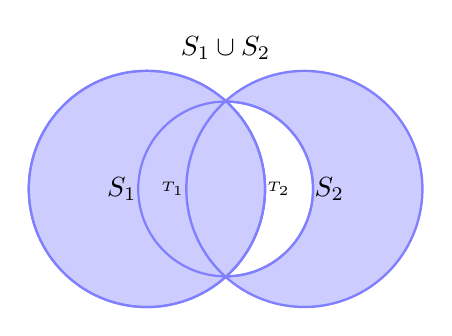
\begin{tikzpicture}
  \draw[filled] \firstcircle \nodeA;
    \begin{scope}
        \clip \secondcircle;
        \draw[filled, even odd rule] \firstcircle \nodeA
                                 \secondcircle 
                                 \thirdcircle;
   \end{scope}
    \draw[outline] \firstcircle
                   \secondcircle \nodeB
                   \thirdcircle \nodeT;

   \node[anchor=south] at (current bounding box.north) {$S_1 \cup S_2$};
\end{tikzpicture}
%Set temporal A or B
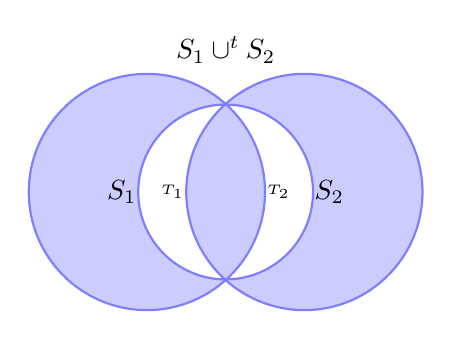
\begin{tikzpicture}
    \draw[filled, even odd rule] \firstcircle \nodeA
                                 \secondcircle \nodeB
                                 \thirdcircle \nodeT;
    \node[anchor=south] at (current bounding box.north) {$S_1 \cup^t S_2$};
\end{tikzpicture}




% Set A but not B
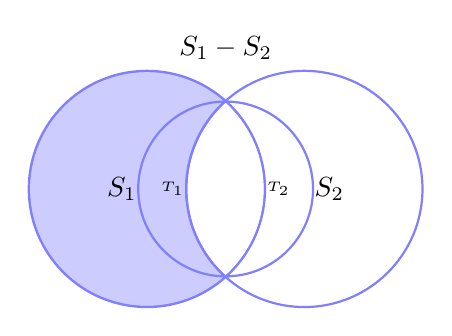
\begin{tikzpicture}
    \begin{scope}
        \clip \firstcircle;
        \draw[filled, even odd rule] \firstcircle \nodeA
                                     \secondcircle;

    \end{scope}
    \draw[outline] \firstcircle
                   \secondcircle \nodeB
                   \thirdcircle \nodeT;
    \node[anchor=south] at (current bounding box.north) {$S_1 - S_2$};
\end{tikzpicture}
% Set temporal A but not B
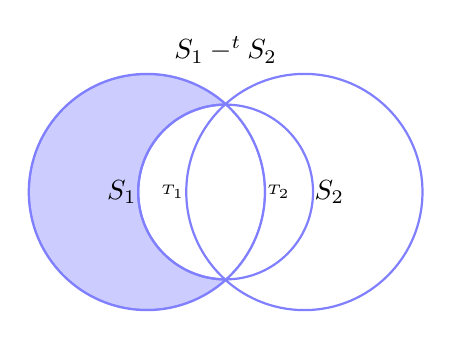
\begin{tikzpicture}
    \begin{scope}
        \clip \firstcircle;
        \draw[filled, even odd rule] \firstcircle \nodeA
                                     \thirdcircle;

    \end{scope}
    \draw[outline] \firstcircle
                   \secondcircle \nodeB
                   \thirdcircle \nodeT;
    \node[anchor=south] at (current bounding box.north) {$S_1 -^t S_2$};
\end{tikzpicture}





% Set A and B
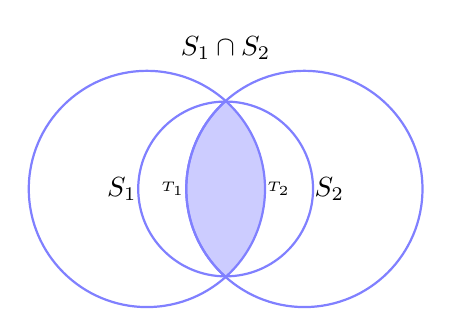
\begin{tikzpicture}
    \begin{scope}
        \clip \firstcircle;
        \fill[filled] \secondcircle;
    \end{scope}
    \draw[outline] \firstcircle \nodeA;
    \draw[outline] \secondcircle \nodeB;
    \draw[outline] \thirdcircle \nodeT;
    \node[anchor=south] at (current bounding box.north) {$S_1 \cap S_2$};
\end{tikzpicture}
% Set temporal A and B
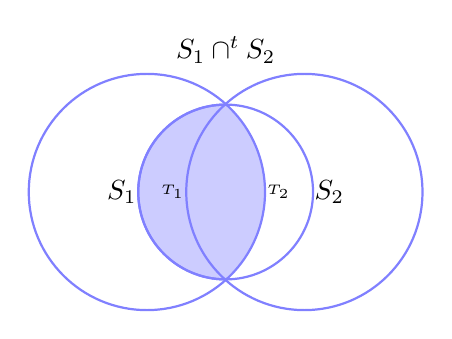
\begin{tikzpicture}
    \begin{scope}
        \clip \firstcircle;
        \fill[filled] \thirdcircle;
    \end{scope}
    \draw[outline] \firstcircle \nodeA;
    \draw[outline] \secondcircle \nodeB;
    \draw[outline] \thirdcircle \nodeT;
    \node[anchor=south] at (current bounding box.north) {$S_1 \cap^t S_2$};
\end{tikzpicture}



%Set A or B but not (A and B) also known a A xor B
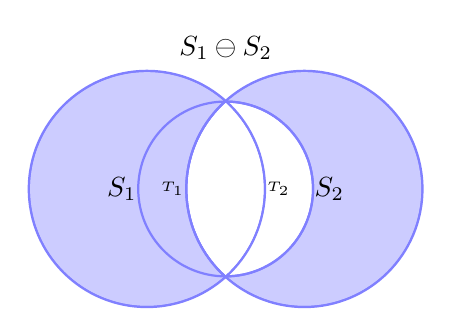
\begin{tikzpicture}
    \begin{scope}
        \clip \firstcircle;
        \draw[filled, even odd rule] \firstcircle
                                     \secondcircle;
    \end{scope}
    \begin{scope}
        \clip \secondcircle;
        \draw[filled, even odd rule] \secondcircle 
                                     \thirdcircle;

    \end{scope}
    \draw[outline] \firstcircle \nodeA;
    \draw[outline] \secondcircle \nodeB;
    \draw[outline] \thirdcircle \nodeT;
    \node[anchor=south] at (current bounding box.north) {$S_1 \ominus S_2$};
\end{tikzpicture}
%Set temporal A or B but not (A and B) also known a A xor B
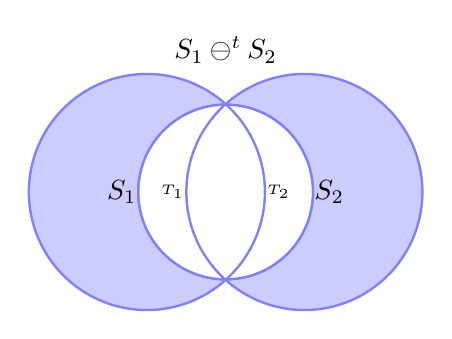
\begin{tikzpicture}
    \begin{scope}
        \clip \firstcircle;
        \draw[filled, even odd rule] \firstcircle
                                     \thirdcircle;
    \end{scope}
    \begin{scope}
        \clip \secondcircle;
        \draw[filled, even odd rule] \secondcircle 
                                     \thirdcircle;

    \end{scope}
    \draw[outline] \firstcircle \nodeA;
    \draw[outline] \secondcircle \nodeB;
    \draw[outline] \thirdcircle \nodeT;
    \node[anchor=south] at (current bounding box.north) {$S_1 \ominus^t S_2$};
\end{tikzpicture}